\documentclass{article}
\usepackage{graphicx} % Required for inserting images
\usepackage{hanging}
\usepackage{amsthm,amsmath,amssymb,amsfonts}
\setlength{\parskip}{5pt}
\usepackage{indentfirst} 
\usepackage[margin=1in]{geometry}
\usepackage{float}
\usepackage[utf8]{inputenc}
\usepackage{setspace}
\usepackage{graphicx}
\usepackage{subcaption}
\usepackage{float}
\usepackage{graphicx}
\usepackage{booktabs}
\usepackage{threeparttable}
\usepackage{natbib}


\title{\textbf{Spatial Patterns and Socioeconomic Determinants\\ of Firearm Violence Across Toronto}}
\author{Nevena Ciganovic}
\date{December 2025}

\begin{document}

\maketitle

\section{Introduction}

\noindent The safety of urban communities is a significant issue for politicians, residents, and scholars, as it reflects not only how well the police do their jobs, but also the underlying social and spatial patterns of the neighborhoods in which people reside. Violent crimes, particularly those involving firearms, are a major factor that influences the safety of a community. We are constantly witnessing or hearing incidents on the news, social media, or among social circles. These types of crime, however, does not occur at random. Spatial crime research shows that violent incidents are geographically concentrated and closely linked to neighbourhood context. Spatial crime research shows that violent incidents are geographically concentrated and closely linked to neighbourhood context \citep{liu2016changchun,zhou2023london}. In Toronto, Statistics Canada documents substantial spatial clustering in police-reported crime and its association with local socioeconomic characteristics \citep{charron2009toronto}.


\noindent Toronto, with its densely populated and diverse urban landscape, offers a great framework for analyzing the impact of social structure and spatial characteristics on crime trends. By examining these trends using spatial tools, this project aims to identify areas in Toronto where instances of firearm violence escalate, determine whether these patterns are statistically significant, and look at whether neighborhood socioeconomic characteristics and observed firearm violence rates are associated. Understanding these relationships may help put public safety concerns in perspective and add to continuing talks about inequality, resource distribution, and community-level action.

\noindent To address these concerns, this project will apply various spatial statistical techniques to uncover spatial patterns and socioeconomic determinants of crime across Toronto. Specifically, we will focus on three research questions:

\begin{enumerate}
    \item Are firearm violence incidents spatially clustered across Toronto, or consistent with complete spatial randomness?
    \item How do firearm violence rates vary across community districts, and are there statistically significant high-crime “hotspots” and low-crime “coldspots”?
    \item How are firearm violence rates associated with neighborhood socioeconomic characteristics after accounting for spatial dependence?
\end{enumerate}

\noindent By integrating point pattern analysis, areal analysis, and spatial regression modeling, this report contributes to the empirical literature on urban crime by demonstrating how firearm violence in Toronto exhibits structured spatial patterns across multiple scales. Rather than treating crime as a purely individual or random phenomenon, the analysis emphasizes the importance of spatial context in understanding and interpreting patterns of firearm violence in urban environments.

\section{Data}

\noindent To answer the above questions of interest, we use three publicly available datasets for the City of Toronto.

\subsection{Shooting and Firearm Discharge Incidents}

\noindent \noindent The \textit{Shooting and Firearm Discharge Incidents} dataset is obtained from the Toronto Police Service Open Data portal \citep{tps_shootings_open_data} and forms the foundation of this project. It contains incident-level records of firearm-related violence in Toronto from 2004 to the present. For this analysis, we extract the following variables:
\begin{itemize}
    \item \texttt{NEIGHBOURHOOD\_158}, indicating the neighbourhood in which the incident occurred;
    \item \texttt{LAT\_WGS84} and \texttt{LONG\_WGS84}, providing the geocoded latitude and longitude of each incident.
\end{itemize}

\noindent Firearm incidents are first mapped as a spatial point pattern and subsequently aggregated to neighbourhoods in order to compute neighbourhood-level shooting counts and rates.

\subsection{Toronto Neighbourhood Boundaries}

\noindent \noindent Neighbourhood boundary data are obtained from the City of Toronto Open Data portal \citep{city_toronto_neighbourhoods}.
Toronto is divided into 158 official neighbourhoods that are commonly used for municipal planning and public reporting. The neighbourhood boundary shapefile provides polygon geometries, which are used to spatially join firearm incident points to neighbourhoods and to construct neighbourhood-level shooting counts and rates.

\subsection{2021 Neighbourhood Profiles}

\noindent \noindent Neighbourhood-level socioeconomic characteristics are obtained from the City of Toronto’s 2021 Neighbourhood Profiles \citep{city_toronto_neighbourhood_profiles}, which summarize demographic and socioeconomic indicators from the 2021 Canadian Census. These data allow us to examine how neighbourhood social context relates to variation in firearm violence. The following variables are used in the analysis:
\begin{itemize}
    \item \texttt{population\_total}, defined as the total neighbourhood population (constructed as total visible minority population plus not a visible minority)
    \item \texttt{median\_total\_income}, the median total household income in 2020
    \item \texttt{unemploy\_rate}, the unemployment rate (percentage);
    \item \texttt{pct\_visible\_minority}, the percentage of residents identifying as a visible minority
    \item \texttt{pct\_black}, the percentage of residents identifying as black
\end{itemize}

\noindent These variables provide the population denominators used to compute shooting rates per 10{,}000 residents and are later incorporated into spatial regression models to evaluate associations between neighbourhood socioeconomic characteristics and firearm violence rates.

\subsection{Data Preprocessing}

\noindent To ensure consistency across datasets and to create neighbourhood-level firearm violence rates suitable for spatial analysis, several preprocessing steps were taken.

\noindent Firearm incident records were filtered to include only observations with valid geographic coordinates. These coordinates were then converted into a spatial point object using the WGS84 coordinate reference system. Toronto neighbourhood boundary polygons were also transformed to the same CRS. All distance-based analyses were conducted using a projected system (UTM Zone 17N).

\noindent Neighbourhood identifiers differed in formatting across data sources. To ensure accurate joins, names were standardized by converting to lowercase, removing accents and punctuation, and collapsing whitespace. This standardized key was used to merge police, boundary, and census-derived datasets.

\noindent Firearm incidents were treated as a spatial point pattern and assigned to neighbourhood polygons via spatial join. Incident counts were then aggregated to the neighbourhood level. Population totals were constructed from the 2021 Neighbourhood Profiles as the sum of visible minority and non–visible minority populations, providing denominators for rate calculations.

\noindent To account for variation in neighbourhood size, firearm violence was expressed as a rate per 10{,}000 residents:
\[
\text{Rate per 10,000} = \frac{\text{Number of firearm incidents}}{\text{Neighbourhood population}} \times 10,000.
\]
This rate serves as the primary outcome for areal analyses and spatial regression models.

\noindent Socioeconomic covariates were converted to proportions where appropriate, and population size was log-transformed to reduce skewness. Missing covariate values were imputed using neighbourhood-level medians to retain all neighbourhoods in the analysis and residual mapping.

\noindent These preprocessing steps ensure that all datasets are spatially aligned, consistent, and scaled for point pattern analysis, areal clustering, and spatial regression modelling.


\section{Methodology}

\noindent This project uses a multi-scale spatial analysis framework to examine firearm violence in Toronto. The methodology is organized into three stages that align with the research questions: (i) point pattern analysis to test whether firearm incidents are spatially clustered, (ii) neighbourhood-level areal analysis to identify spatial dependence and local clusters in shooting rates, and (iii) spatial regression modelling to assess socioeconomic associations while accounting for spatial dependence.

\subsection{Point Pattern Analysis}

\noindent To assess whether firearm incidents are consistent with complete spatial randomness (CSR), incidents were first treated as a spatial point pattern within the city boundary. Under CSR, events are assumed to arise from a homogeneous Poisson process with constant intensity $\lambda$, implying spatial independence and no interaction between points.

\noindent Formally, CSR implies
\[
N(A) \sim \text{Poisson}(\lambda |A|),
\]
where $N(A)$ is the number of events in region $A$ and $|A|$ denotes its area. Deviations from CSR were evaluated using second-order summary statistics.

\noindent Ripley’s $K$-function and its variance-stabilized transformation $L(r) = \sqrt{K(r)/\pi}$ were used to examine clustering across spatial scales. Under CSR, $L(r) = r$. Values of $L(r) > r$ indicate clustering, while $L(r) < r$ indicates inhibition. In addition, the nearest-neighbour distribution function $G(r)$ was used to assess short-range interaction, with faster-than-expected increases at small distances indicating clustering.

\noindent Statistical significance was assessed using Monte Carlo simulation envelopes generated under CSR. Global envelope tests were used to control for multiple testing across distances. Rejection of CSR motivates the use of intensity-based visualization and areal aggregation in subsequent analyses.

\subsection{Kernel Density Estimation}

\noindent Following rejection of CSR, kernel density estimation (KDE) was used to visualize spatial variation in the intensity of firearm incidents. KDE estimates the spatial intensity function $\lambda(s)$ as
\[
\hat{\lambda}(s) = \sum_{i=1}^{n} \frac{1}{2\pi\sigma^2}
\exp\left(-\frac{\|s - x_i\|^2}{2\sigma^2}\right),
\]
where $x_i$ denotes event locations and $\sigma$ is the bandwidth controlling the degree of spatial smoothing.

\noindent Multiple bandwidths were examined to illustrate clustering at different spatial scales, including a data-driven bandwidth and fixed bandwidths corresponding to local and regional scales. KDE results are used descriptively and not as inputs to later models, serving instead to contextualize neighbourhood-level patterns examined in RQ2.

\subsection{Areal Analysis and Spatial Autocorrelation}

\noindent To examine spatial structure at the neighbourhood level, firearm incidents were aggregated to Toronto’s 158 official neighbourhoods and converted to shooting rates per 10{,}000 residents. This aggregation shifts the analysis from point-level events to areal outcomes, allowing the use of spatial autocorrelation statistics.

\subsubsection{Spatial Weights}

\noindent
Spatial dependence was defined using three alternative neighbourhood structures: Queen contiguity, Rook
contiguity, and a symmetric $k$-nearest-neighbour graph with $k=18$. Queen contiguity defines neighbours as
polygons sharing either an edge or a vertex, while Rook contiguity restricts neighbours to shared edges
only. The $k$NN structure instead defines neighbourhoods based on geographic proximity between centroids,
ensuring a fixed number of neighbours for each area.

\noindent
All three weighting schemes produced connected spatial graphs and yielded similar patterns of spatial
autocorrelation. Queen contiguity was selected for primary inference due to its interpretability and its
consistency with administrative neighbourhood boundaries.


\subsubsection{Global Spatial Autocorrelation}

\noindent Global spatial dependence was assessed using Moran’s $I$, defined as
\[
I = \frac{n}{\sum_{i}\sum_{j} w_{ij}}
\frac{\sum_{i}\sum_{j} w_{ij}(y_i - \bar{y})(y_j - \bar{y})}
{\sum_{i}(y_i - \bar{y})^2},
\]
where $y_i$ is the shooting rate in neighbourhood $i$ and $w_{ij}$ are spatial weights. Under the null hypothesis of spatial randomness, $E[I] = -(n-1)^{-1}$. Moran’s $I$ was computed under each weighting scheme to assess robustness to neighbourhood definition.

\subsubsection{Local Indicators of Spatial Association}

\noindent
To identify where clustering occurs, Local Moran’s $I$ (LISA) and the Getis--Ord $G_i^*$ statistic were computed using Queen contiguity weights. LISA decomposes global spatial autocorrelation into location-specific contributions, identifying neighbourhoods participating in statistically significant high--high and low--low clusters, while the $G_i^*$ statistic detects local hot and cold spots based on concentrations of high or low values. Holm-adjusted $p$-values were used to control for multiple local tests.

\subsection{Spatial Regression Modelling}

\noindent Motivated by the presence of spatial autocorrelation in neighbourhood shooting rates, we modelled rates as a function of socioeconomic covariates while explicitly accounting for spatial dependence.

\subsubsection{Ordinary Least-Squares Model}

\noindent The baseline model is an ordinary least squares (OLS) regression of the form
\[
y = X\beta + \varepsilon,
\]
where $y$ is the shooting rate per 10{,}000 residents and $X$ includes median household income, unemployment rate, proportion of visible minority residents, proportion of Black residents, and log population. Standard OLS assumptions include independent and identically distributed errors; violations of these assumptions are assessed using Moran’s $I$ on residuals.

\subsubsection{Spatial Regression Models}

\noindent To address residual spatial dependence, several spatial regression models were estimated:

\begin{itemize}
    \item \textbf{Spatial Error Model:}
    \[
    y = X\beta + u, \quad u = \lambda Wu + \varepsilon,
    \]
    capturing spatial correlation in unobserved factors.

    \item \textbf{Spatial Lag Model:}
    \[
    y = \rho Wy + X\beta + \varepsilon,
    \]
    allowing outcomes in neighbouring areas to directly influence each other.

    \item \textbf{Spatial Lag-Error Model:} combining both lag and error dependence.

    \item \textbf{Conditional Autoregressive (CAR) Model:} estimated using binary contiguity weights, modelling neighbourhood outcomes as conditionally dependent on adjacent areas.
\end{itemize}

\subsubsection{Model Diagnostics and Comparison}

\noindent Model adequacy was assessed using Akaike’s Information Criterion (AIC) and Moran’s $I$ on model residuals. Rao’s score (LM) tests were applied to the OLS model to diagnose the form of spatial dependence and guide model choice. Residual maps were used as a diagnostic visualization to assess whether spatial structure was effectively absorbed by each model.

\noindent Together, these methods help prevent the misinterpretation of socioeconomic relationships caused by spatial dependencies that are not accounted for. They also allow for a systematic comparison of different spatial models.


\section{Results}

\subsection{Exploratory Spatial Patterns of Firearm Incidents}
\noindent Before formal spatial modeling, we first explore the geographic distribution of firearm incidents across Toronto to gain intuition about the spatial structure of the data.

\begin{figure}[H]
\centering
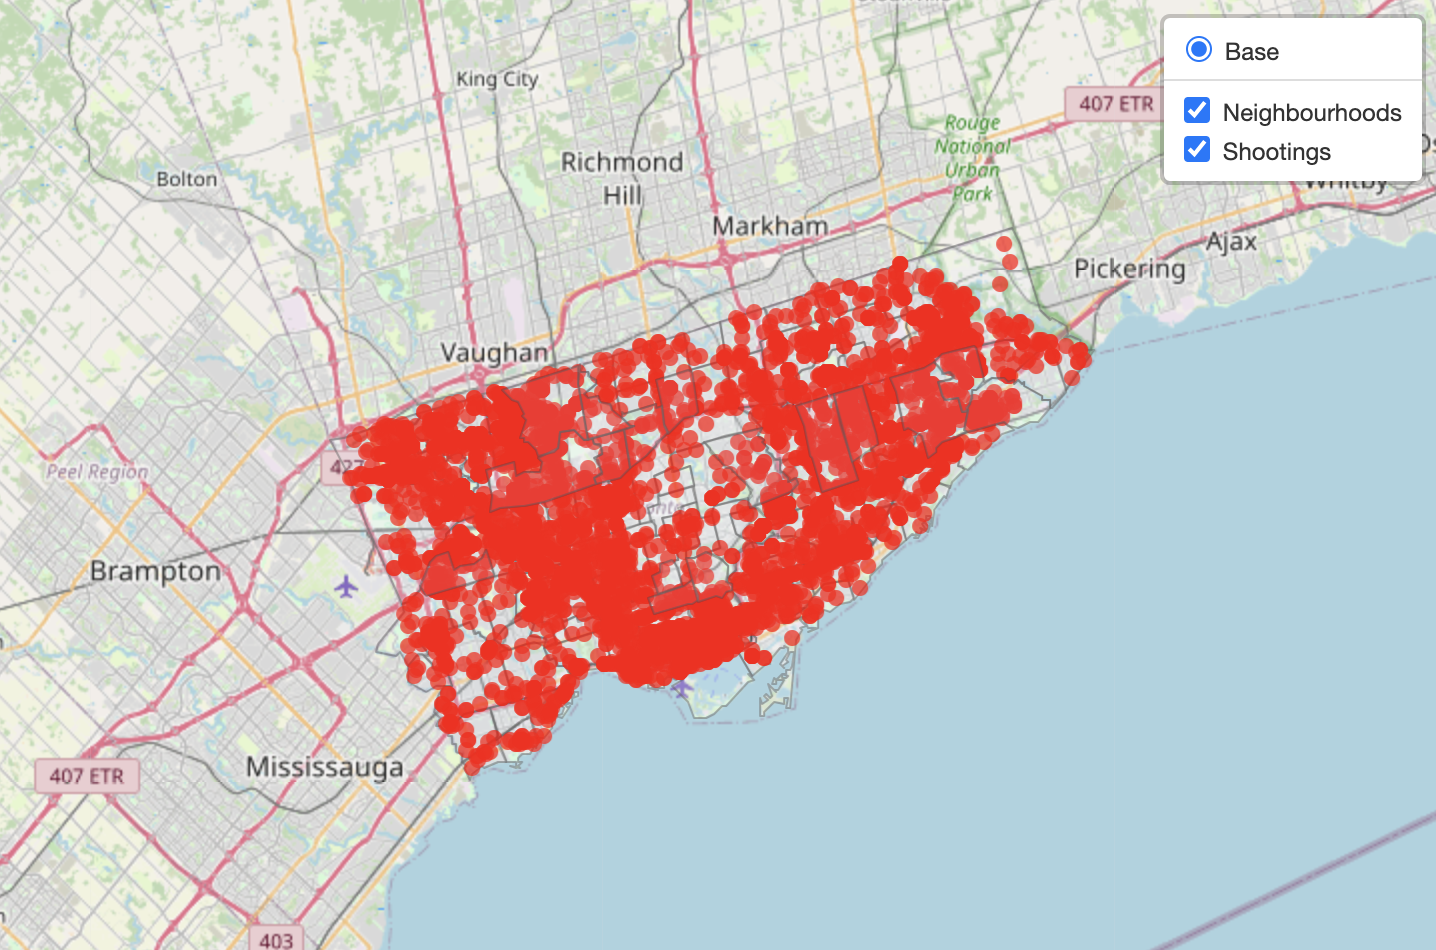
\includegraphics[scale=0.3]{fig1.png}
\caption{Map of shooting incidents and neighbourhood boundaries}
\end{figure}

\noindent Figure 1 displays the spatial distribution of firearm discharge incidents across the City of Toronto overlaid on neighbourhood boundaries. Incidents are widely distributed across the city but are visibly more concentrated in certain parts of the urban core and western portions of Toronto. This exploratory visualization suggests that firearm incidents are not evenly distributed in space and motivates a formal point pattern analysis to assess whether this apparent clustering is statistically significant.

\begin{figure}[H]
\centering
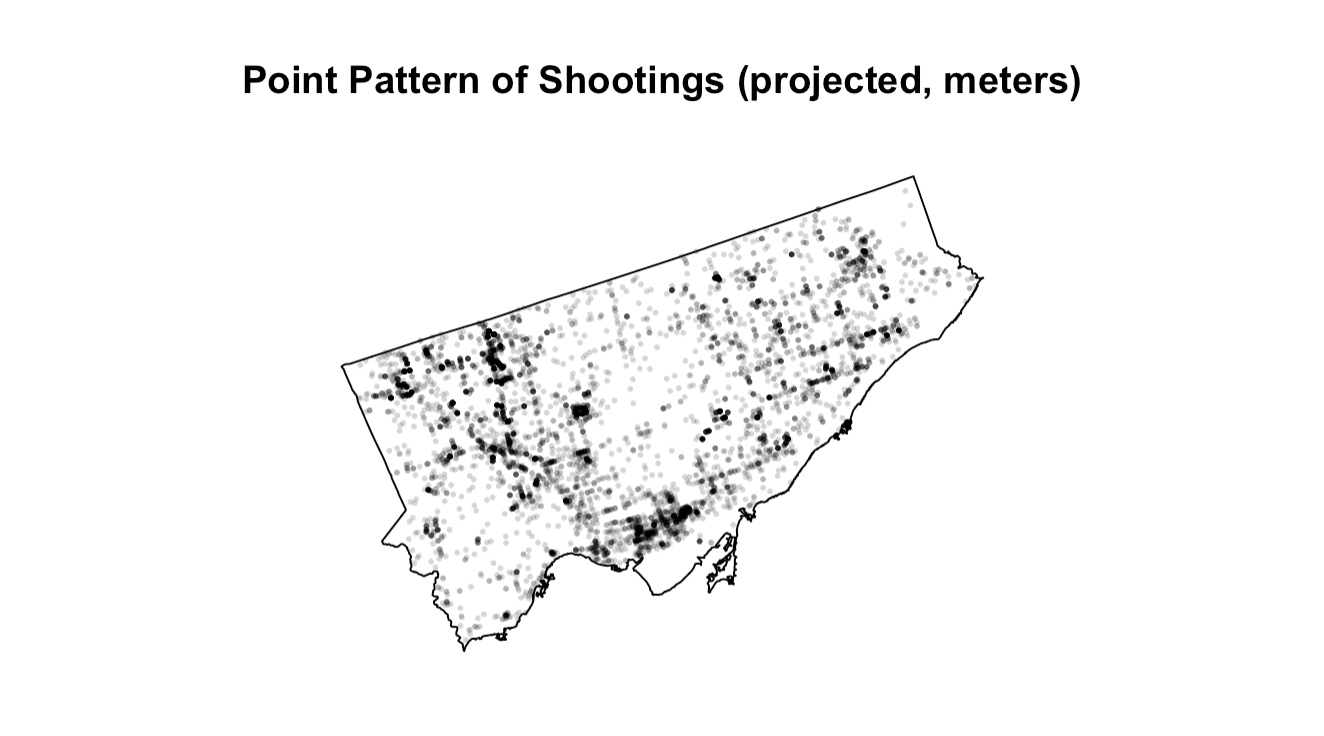
\includegraphics[scale=0.4]{fig2.png}
\caption{Static projected point pattern of shootings}
\end{figure}

\noindent To support subsequent spatial analyses, incident locations were projected into a planar coordinate system (UTM Zone 17N) and visualized as a point pattern. This representation allows distances to be interpreted in meters and serves as the basis for complete spatial randomness (CSR) testing and kernel density estimation.

\subsection{Are Firearm Violence Incidents Spatially Clustered?}

\subsubsection{Testing Complete Spatial Randomness}

\noindent To formally assess whether firearm incidents are consistent with complete spatial randomness (CSR), we applied global second-order point pattern diagnostics using Ripley’s $L(r)$ function and the nearest-neighbor $G(r)$ function. Monte Carlo envelopes were generated under CSR using repeated simulations of a homogeneous Poisson process.

\begin{figure}[H]
    \centering
    \begin{subfigure}[t]{0.32\textwidth}
        \centering
        % INSERT L(r)-r plot
        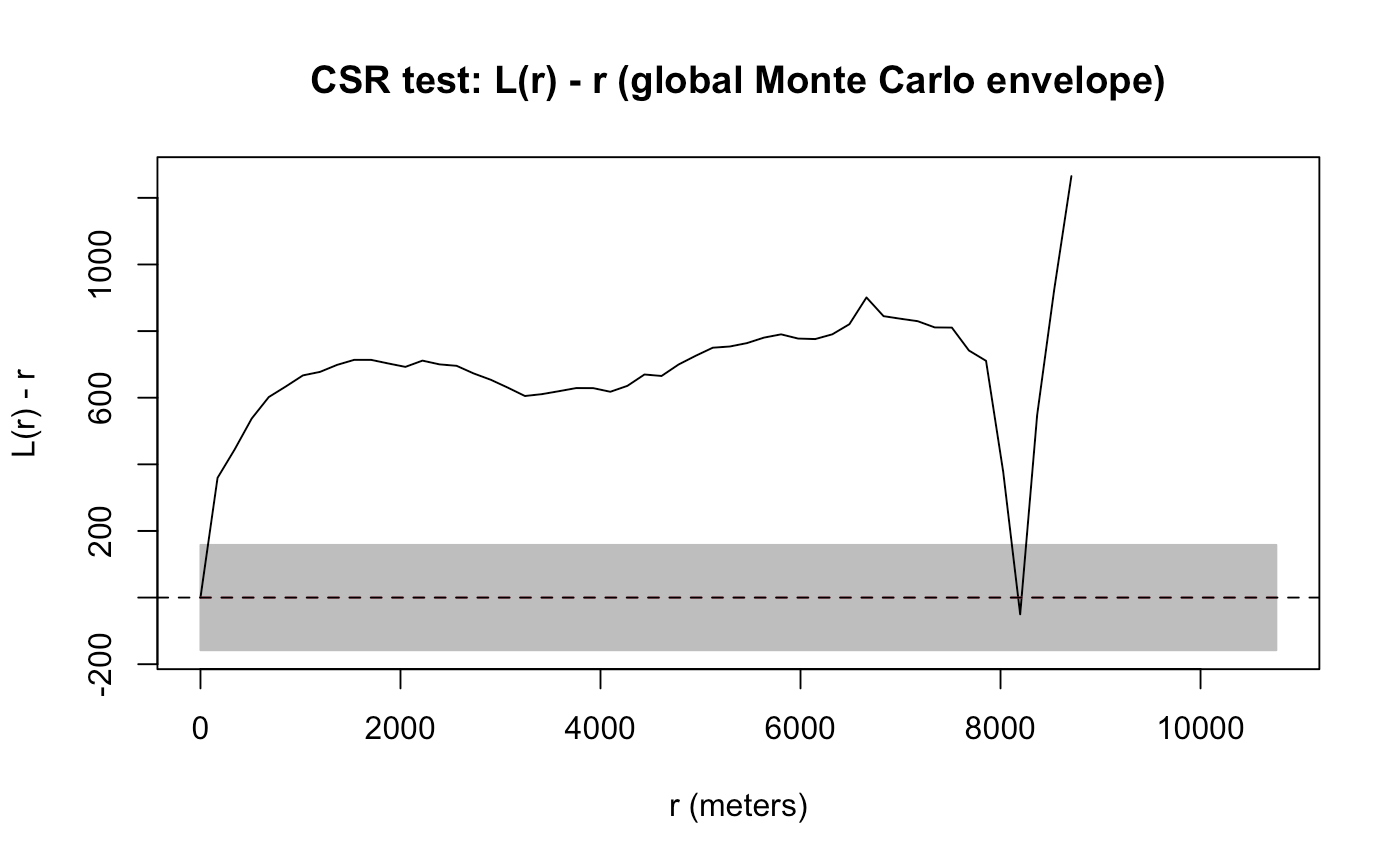
\includegraphics[width=\textwidth]{fig3.png}
        \caption{$L(r)-r$ envelope}
    \end{subfigure}
    \hspace{1 cm}
    \begin{subfigure}[t]{0.32\textwidth}
        \centering
        % INSERT G(r) plot
        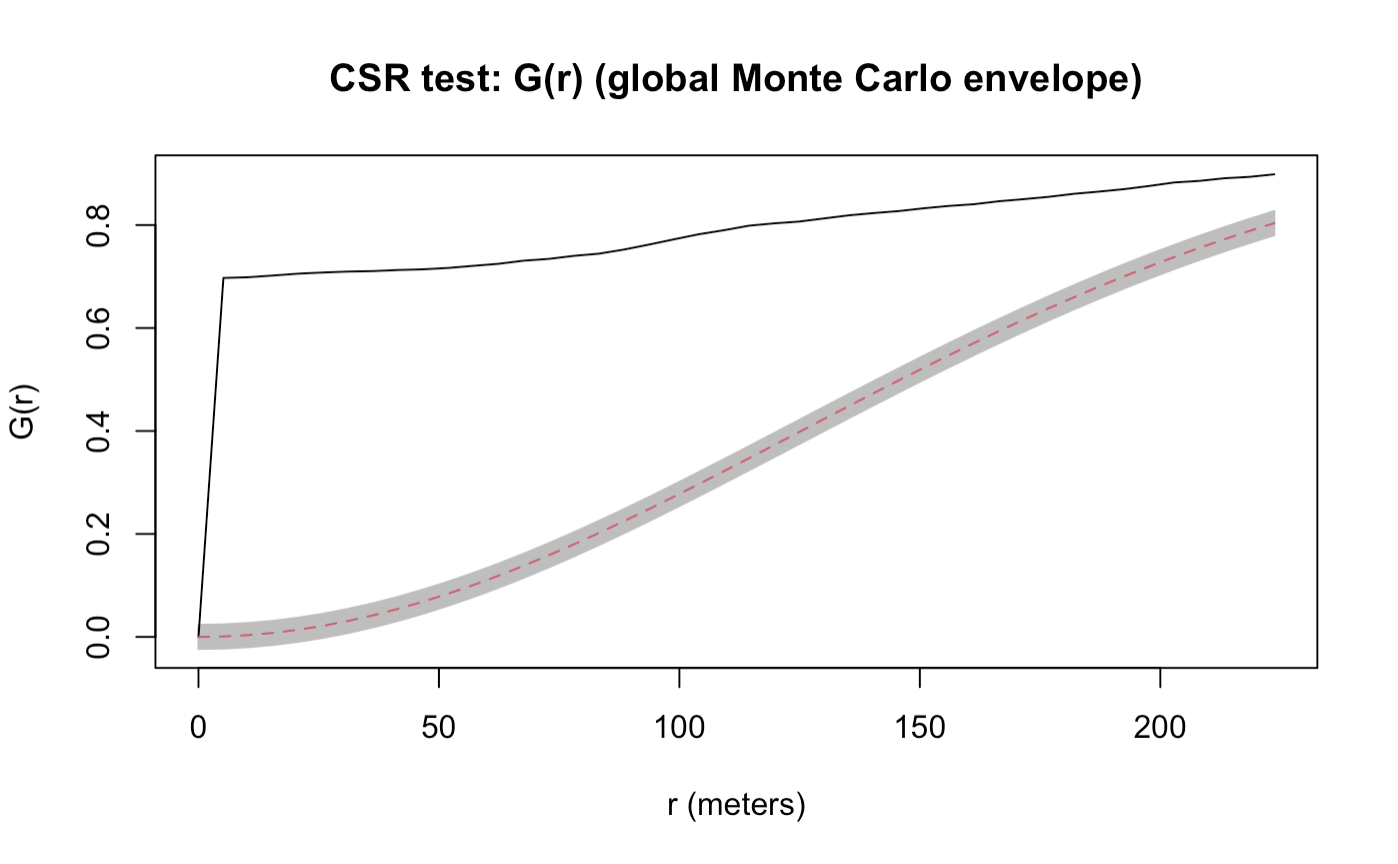
\includegraphics[width=\textwidth]{fig4}
        \caption{$G(r)$ envelope}
    \end{subfigure}
    
    \caption{Tests of complete spatial randomness (CSR) for firearm incidents in Toronto.}
    \label{fig:csr_combined}
\end{figure}

\noindent Figure~\ref{fig:csr_combined} provides consistent evidence against complete spatial randomness. 
In panel (a), the empirical $L(r)-r$ curve lies well above the simulation envelope across a wide range of distances, indicating clustering beyond CSR. 
Panel (b) shows that the observed $G(r)$ rises more rapidly than expected at short distances, reflecting an excess of nearby events. 
These results demonstrate strong spatial clustering of firearm incidents across multiple spatial scales.

\subsubsection{Kernel Density Estimation}

\noindent Given the rejection of CSR, kernel density estimation (KDE) was used to visualize the spatial intensity of firearm incidents across Toronto. KDE surfaces were computed using multiple bandwidths to illustrate clustering at different spatial scales.

\begin{figure}[H]
    \centering
    \begin{subfigure}[t]{0.32\textwidth}
        \centering
        % INSERT KDE auto bandwidth
        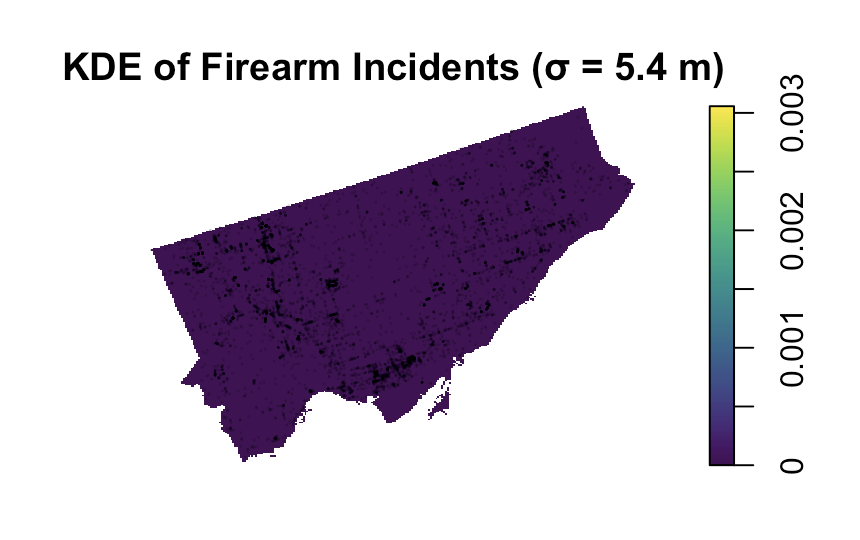
\includegraphics[width=\textwidth]{fig5.png}
        \caption{Data-driven bandwidth}
    \end{subfigure}
    \hfill
    \begin{subfigure}[t]{0.32\textwidth}
        \centering
        % INSERT KDE 500m
        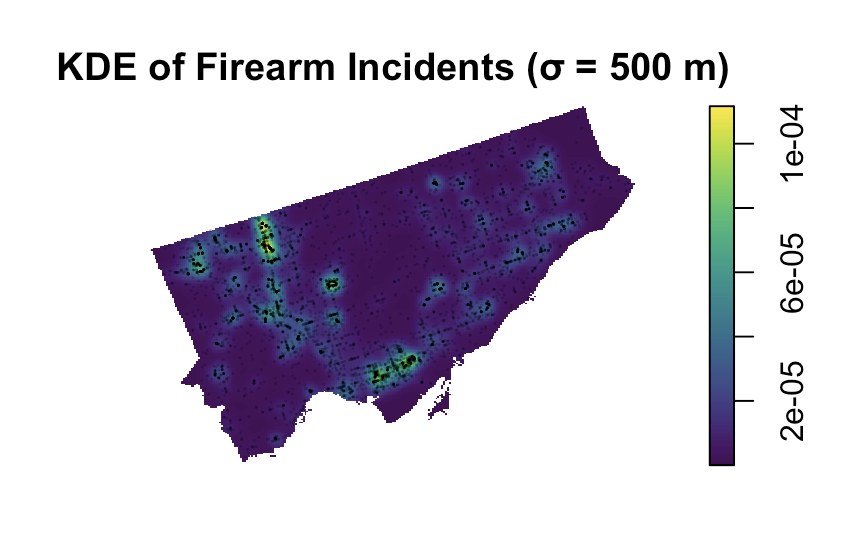
\includegraphics[width=\textwidth]{fig6.png}
        \caption{$\sigma = 500$ m}
    \end{subfigure}
    \hfill
    \begin{subfigure}[t]{0.32\textwidth}
        \centering
        % INSERT KDE 2000m
        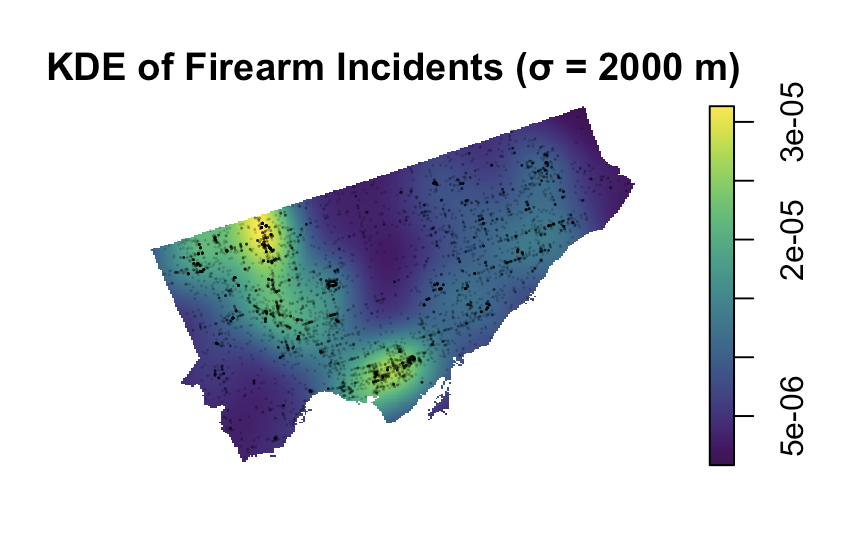
\includegraphics[width=\textwidth]{fig7.png}
        \caption{$\sigma = 2000$ m}
    \end{subfigure}

    \caption{Kernel density estimates (KDE) of firearm incidents at multiple spatial scales.}
    \label{fig:kde_combined}
\end{figure}

\noindent Figure~\ref{fig:kde_combined} illustrates how spatial clustering of firearm incidents varies across scales. Consistent with the CSR tests, elevated intensity appears concentrated in a limited set of areas rather than being evenly distributed across the city. This motivates the neighbourhood-level hotspot analysis in RQ2.

\subsection{Neighbourhood Variation in Shooting Rates}

\noindent Motivated by the rejection of complete spatial randomness in RQ1, we next shift from the point-level incident pattern to an areal (neighbourhood-level) view to understand how firearm violence rates vary across Toronto and whether high-rate and low-rate areas form statistically meaningful clusters. Figure~\ref{fig:rq2_rates} shows that neighbourhoods in the upper quintiles of shooting rates are not evenly scattered across the city but appear spatially concentrated, suggesting that neighbourhood-level dependence remains after aggregation.

\begin{figure}[H]
  \centering
  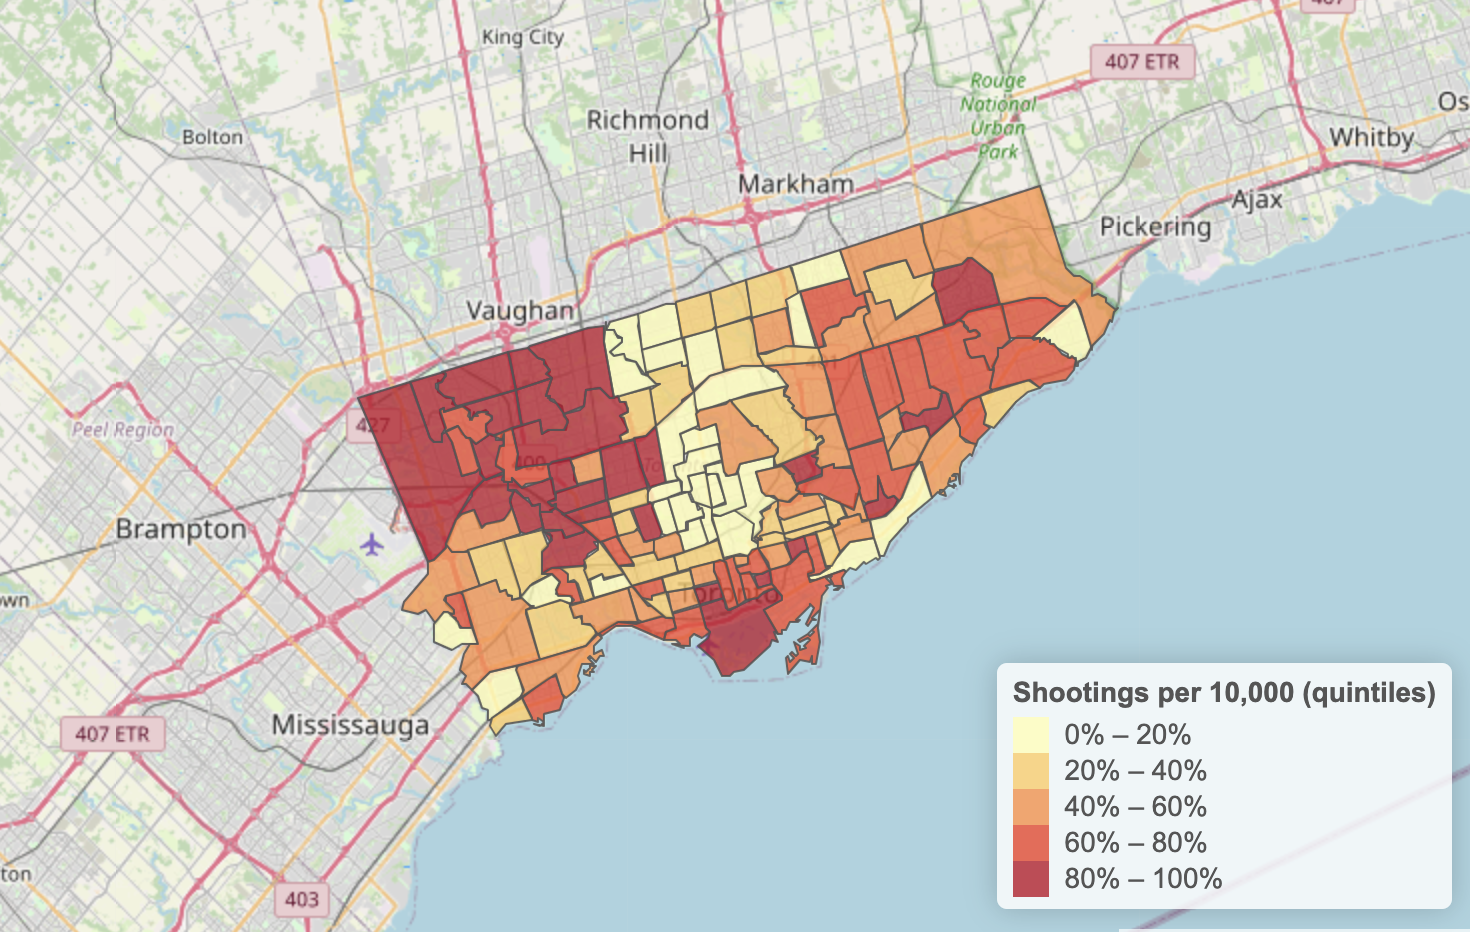
\includegraphics[scale=0.3]{fig8.png}
  \caption{Neighbourhood shooting rates per 10{,}000 residents (quintiles).}
  \label{fig:rq2_rates}
\end{figure}

\subsubsection{Neighbourhood structure and choice of spatial weights}

\noindent We compared three common weight structures: Queen contiguity, Rook contiguity, and a symmetric $k$-nearest-neighbour graph with $k=18$. All three graphs were connected (one connected component), but they differ in density: Queen is slightly denser than Rook, while $18$-NN is substantially denser due to the forced minimum degree. These differences matter because they change the scale at which nearby neighbourhoods influence each other.

\begin{figure}[H]
\centering
\begin{subfigure}[t]{0.32\textwidth}
  \centering
  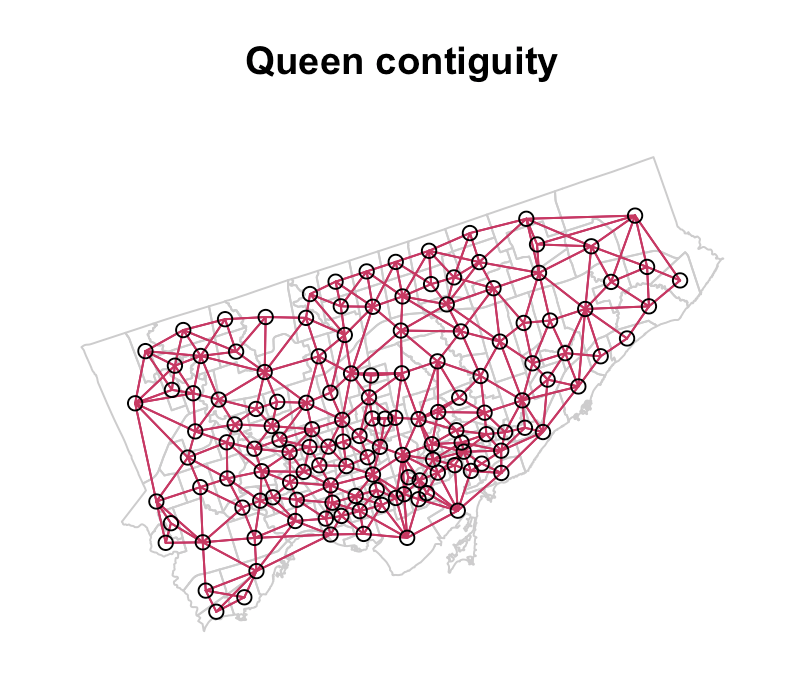
\includegraphics[width=\textwidth]{fig9.png}
  \small (a) Queen contiguity
\end{subfigure}
\begin{subfigure}[t]{0.32\textwidth}
  \centering
  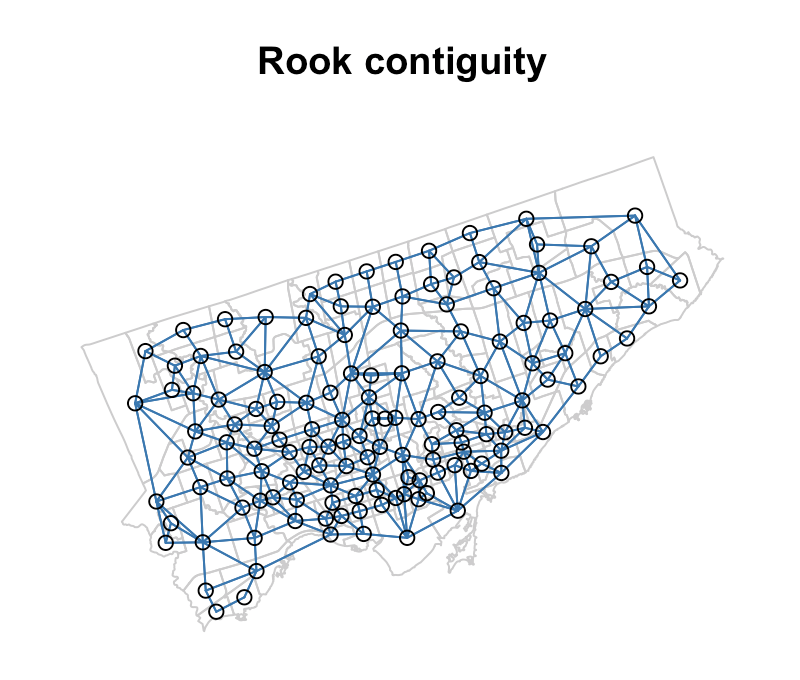
\includegraphics[width=\textwidth]{fig10.png}\\[-2mm]
  \small (b) Rook contiguity
\end{subfigure}
\begin{subfigure}[t]{0.32\textwidth}
  \centering
  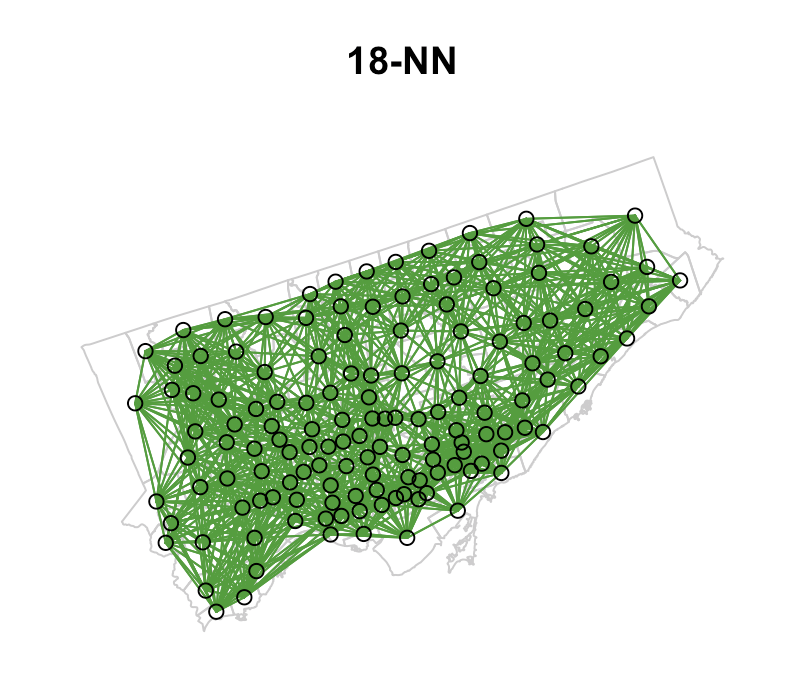
\includegraphics[width=\textwidth]{fig11.png}\\[-2mm]
  \small (c) $18$-nearest neighbours
\end{subfigure}
\caption{Neighbourhood graphs used to define spatial weights.}
\label{fig:rq2_weights_graphs}
\end{figure}

\noindent We then computed Global Moran's $I$ for the shooting rate per 10{,}000 under each weighting scheme. Table~\ref{tab:rq2_weights_summary} shows that spatial autocorrelation is strongly positive under all three structures, supporting the visual impression of clustering in Figure~\ref{fig:rq2_rates}. Queen and Rook produce very similar estimates, while the denser $18$-NN graph yields a smaller $I$ (as expected when neighbourhood influence is spread across many neighbours). Given the interpretability of contiguity in an areal setting and the similarity between Queen and Rook results, we proceed with Queen contiguity for the remainder of RQ2 (and for later modelling in RQ3).

\begin{table}[H]
\centering
\begin{threeparttable}
\caption{Summary of spatial weights and Global Moran's $I$ for neighbourhood shooting rate per 10{,}000.}
\label{tab:rq2_weights_summary}
\begin{tabular}{lrrrr}
\toprule
Weights & Avg.\ degree & Connected components & Moran's $I$ & $p$-value \\
\midrule
Queen contiguity & 5.971 & 1 & 0.446 & $9.20\times 10^{-21}$ \\
Rook contiguity  & 5.014 & 1 & 0.458 & $3.18\times 10^{-18}$ \\
$18$-NN (symmetric) & 21.657 & 1 & 0.328 & $1.05\times 10^{-45}$ \\
\bottomrule
\end{tabular}
\begin{tablenotes}[flushleft]
\footnotesize
Notes: Moran's $I$ is computed on the neighbourhood shooting rate per 10{,}000 residents. Average degree is the mean number of neighbours per area (after symmetrization for $k$-NN). P-values correspond to the global Moran test output under each weight structure.
\end{tablenotes}
\end{threeparttable}
\end{table}

\subsubsection{Global dependence and local clusters (LISA and Gi*)}

\begin{figure}[H]
\centering
\begin{subfigure}[t]{0.48\textwidth}
  \centering
  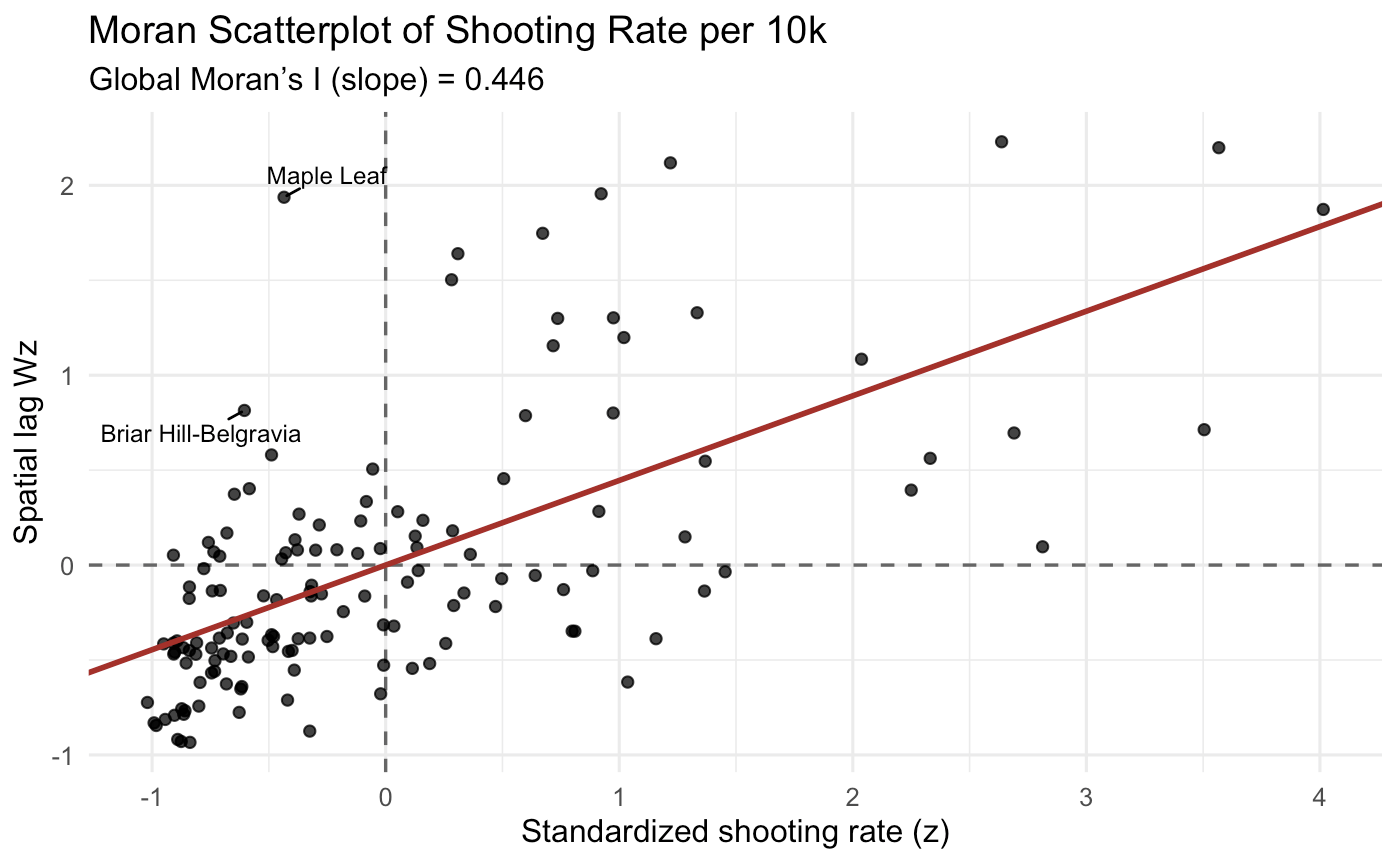
\includegraphics[width=\textwidth]{fig12.png}\\[-2mm]
  \small (a) Moran scatterplot (Queen weights)
\end{subfigure}\hfill
\begin{subfigure}[t]{0.48\textwidth}
  \centering
  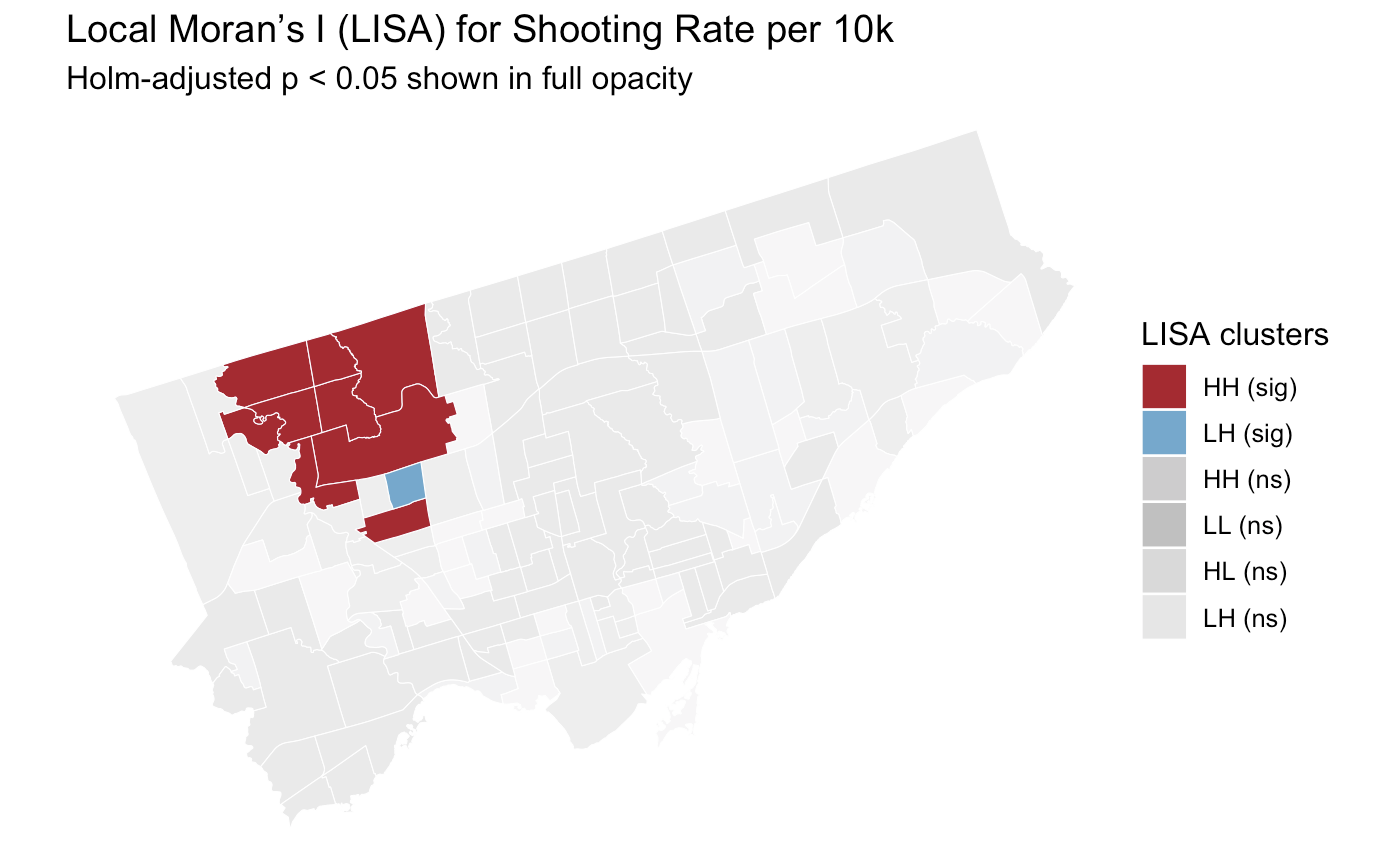
\includegraphics[width=\textwidth]{fig13.png}\\[-2mm]
  \small (b) LISA cluster map (Holm-adjusted $p<0.05$)
\end{subfigure}

\vspace{5mm}

\begin{subfigure}[t]{0.48\textwidth}
  \centering
  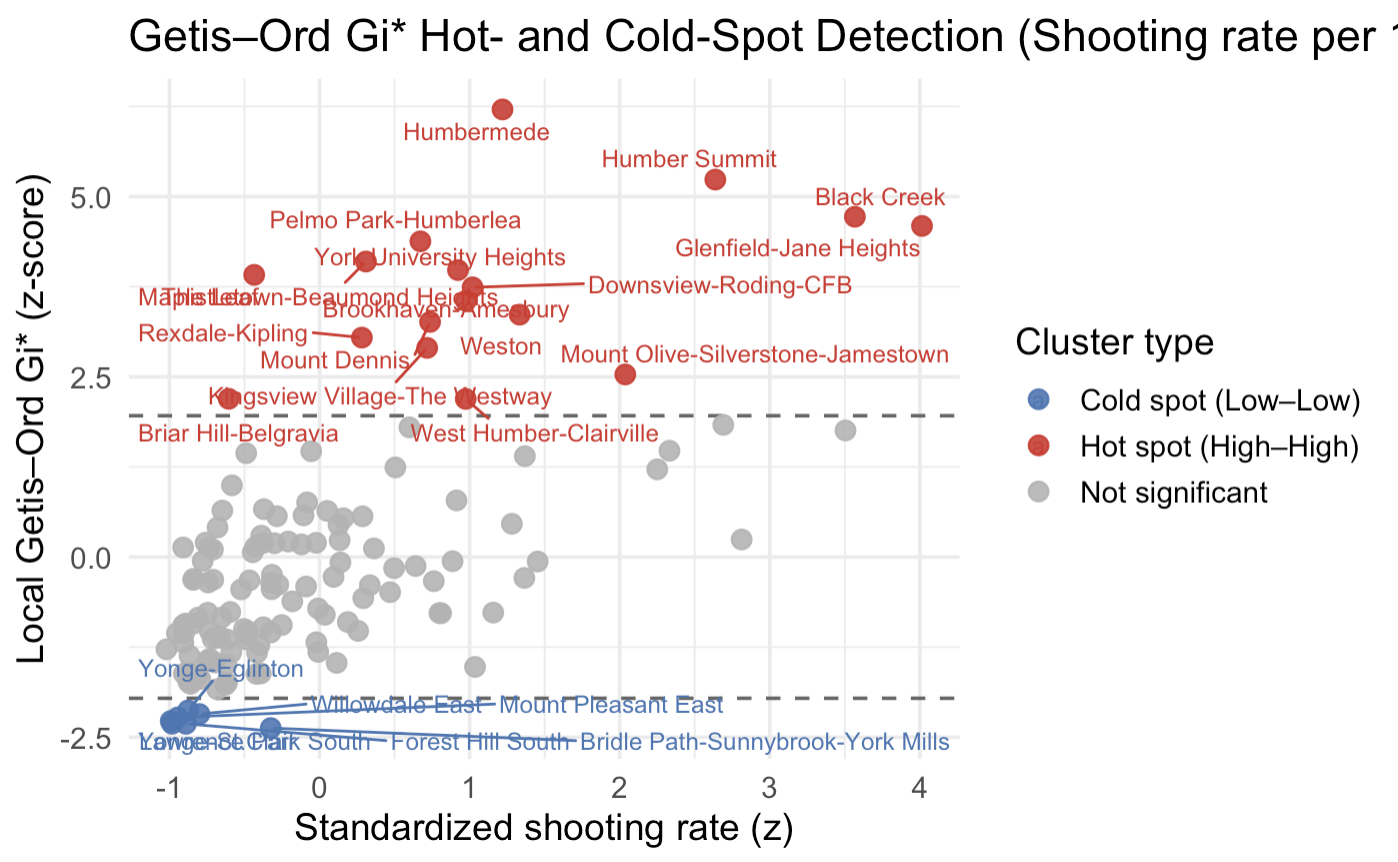
\includegraphics[width=\textwidth]{fig14.png}\\[-2mm]
  \small (c) Getis--Ord $G_i^*$ scatterplot
\end{subfigure}\hfill
\begin{subfigure}[t]{0.48\textwidth}
  \centering
  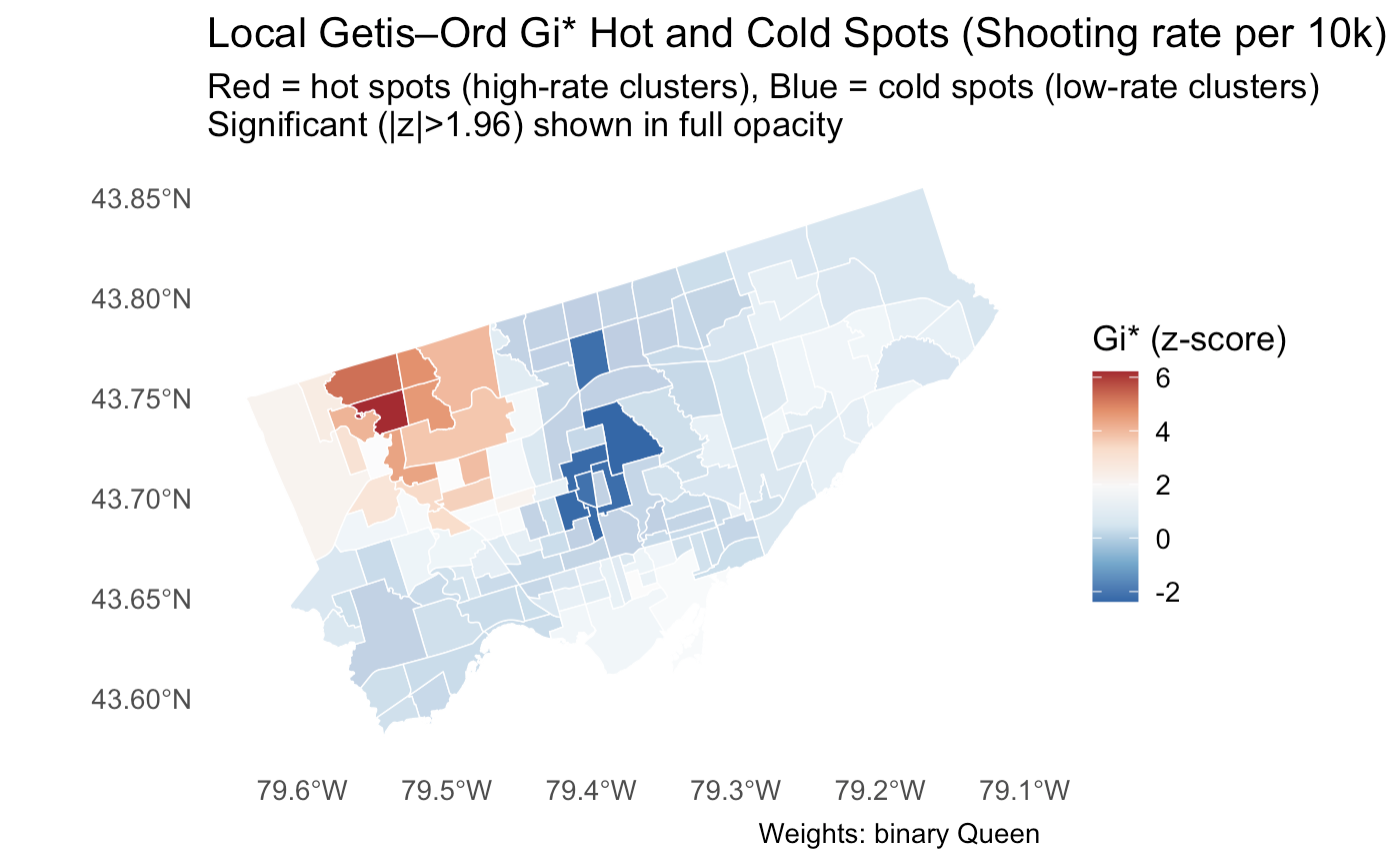
\includegraphics[width=\textwidth]{fig15.png}\\[-2mm]
  \small (d) Getis--Ord $G_i^*$ map (significant areas emphasized)
\end{subfigure}
\caption{Global and local spatial dependence in neighbourhood shooting rates per 10{,}000 (Queen weights).}
\label{fig:rq2_lisa_gi_all}
\end{figure}

\noindent The presence of positive global spatial autocorrelation is reflected in the Moran scatterplot (Figure~\ref{fig:rq2_lisa_gi_all}a), where neighbourhoods with higher-than-average shooting rates tend to be surrounded by neighbours with similarly high rates, and low-rate neighbourhoods tend to be adjacent to other low-rate areas. This pattern confirms that firearm violence rates are spatially clustered rather than randomly distributed across the city.

\noindent Local indicators of spatial association further clarify where this clustering occurs. The Local Moran’s $I$ (LISA) map (Figure~\ref{fig:rq2_lisa_gi_all}b) reveals a contiguous group of neighbourhoods forming a statistically significant high--high cluster, indicating concentrated areas of elevated firearm violence. In contrast, most neighbourhoods outside this region do not exhibit significant local clustering, suggesting that high shooting rates are not widespread but geographically localized.

\noindent The Getis--Ord $G_i^*$ results reinforce this conclusion. The scatterplot (Figure~\ref{fig:rq2_lisa_gi_all}c) highlights neighbourhoods with significantly high and low $z$-scores, while the corresponding map (Figure~\ref{fig:rq2_lisa_gi_all}d) shows that hot spots are confined to a compact area of the city, with cold spots occurring in a separate region characterized by consistently low shooting rates. Together, these results indicate that firearm violence in Toronto exhibits strong local concentration, with distinct neighbourhood clusters rather than diffuse spatial patterns.

\noindent Overall, RQ2 shows that firearm violence rates are not only heterogeneous across neighbourhoods but also spatially dependent, with statistically significant clusters of high and low rates under reasonable neighbourhood definitions. This motivates RQ3, as the strong spatial dependence in shooting rates means that regression models must account for spatial structure to avoid biased inference and to separate socioeconomic associations from residual clustering.

\subsection{Neighbourhood Socioeconomic Factors and Shooting Rates}

\subsubsection{Ordinary Least-Squares}

\noindent Table~\ref{tab:rq3_models} shows that the ordinary least squares (OLS) model explains a substantial portion of the variation in neighbourhood shooting rates ($R^2 = 0.59$). Among the covariates, the proportion of Black residents is the only consistently significant predictor, with higher proportions associated with higher shooting rates. Other socioeconomic variables, including median income, unemployment, housing characteristics, and population size, are not statistically significant.

\noindent Despite the reasonable overall fit, the OLS residuals exhibit significant positive spatial autocorrelation (Moran’s $I = 0.151$, $p < 0.001$), indicating that unexplained spatial structure remains. This pattern is visible in Figure~\ref{fig:rq3_residuals}, where clusters of positive and negative residuals appear spatially grouped rather than randomly distributed.

\begin{table}[ht]
\centering
\caption{Comparison of regression models for neighbourhood shooting rates}
\label{tab:rq3_models}
\begin{tabular}{lcccc}
\hline
Model & AIC & Spatial parameter & Moran’s $I$ (resid.) & $p$-value \\
\hline
OLS & 1165.1 & -- & 0.151 & $<0.001$ \\
SAR Error & 1159.1 & $\lambda = 0.36$ & $-0.009$ & 0.52 \\
SAR Lag & 1158.3 & $\rho = 0.26$ & 0.011 & 0.36 \\
SAR Lag--Error & 1160.1 & $\rho = 0.20$, $\lambda = 00.12$ & $-0.003$ & 0.47 \\
CAR & 1161.0 & $\lambda = 0.10$ & $-0.105$ & 0.98 \\
\hline
\end{tabular}

\vspace{0.5em}
\footnotesize
\textit{Notes:} Moran’s $I$ is computed on model residuals using Queen contiguity weights (binary weights for CAR).
\end{table}

\subsubsection{Spatial Regression Models}

\noindent All spatial models substantially reduce residual spatial autocorrelation relative to OLS (Table~\ref{tab:rq3_models}). In the spatial error model, residual spatial autocorrelation is fully removed (Moran’s $I \approx 0$, $p = 0.52$), and the spatial error parameter is statistically significant. The spatial lag model also eliminates residual autocorrelation and achieves the lowest AIC among all models, suggesting a modest improvement in overall fit.

\noindent The combined lag–error model and the CAR model likewise remove residual spatial dependence, though neither provides a clear improvement over the simpler SAR error or SAR lag based on AIC. Across all spatial specifications, coefficient estimates are stable: the proportion of Black residents remains strongly associated with higher shooting rates, while other covariates remain statistically insignificant.

\noindent Residual maps in Figure~\ref{fig:rq3_residuals} show that spatial models produce smoother, less clustered residual patterns than OLS, indicating that spatial dependence is being effectively absorbed by the model structure.

\subsubsection{Model comparison and diagnostics}

\noindent Table~\ref{tab:rq3_models} summarizes model performance and diagnostic results. Relative to OLS, all spatial models improve fit and eliminate residual spatial autocorrelation. Among them, the SAR lag model achieves the lowest AIC, while the SAR error model provides the cleanest removal of spatial structure with minimal model complexity. Overall, the results indicate that accounting for spatial dependence is essential for valid inference in neighbourhood-level shooting rate models.

\begin{figure}[ht]
\centering

% ---- Row 1: three models ----
\begin{subfigure}{0.32\textwidth}
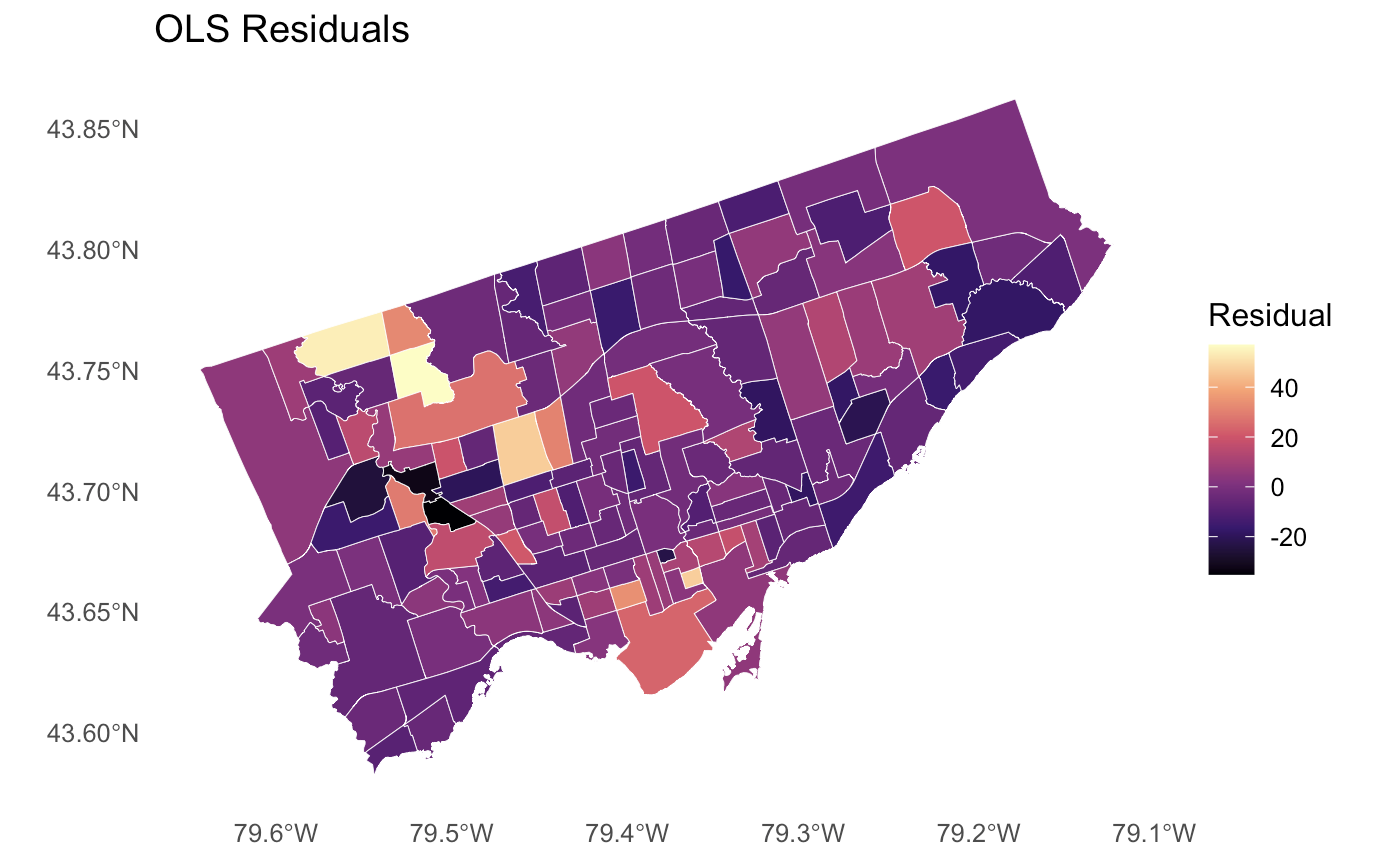
\includegraphics[width=\linewidth]{fig16.png}
\caption{OLS}
\end{subfigure}
\hfill
\begin{subfigure}{0.32\textwidth}
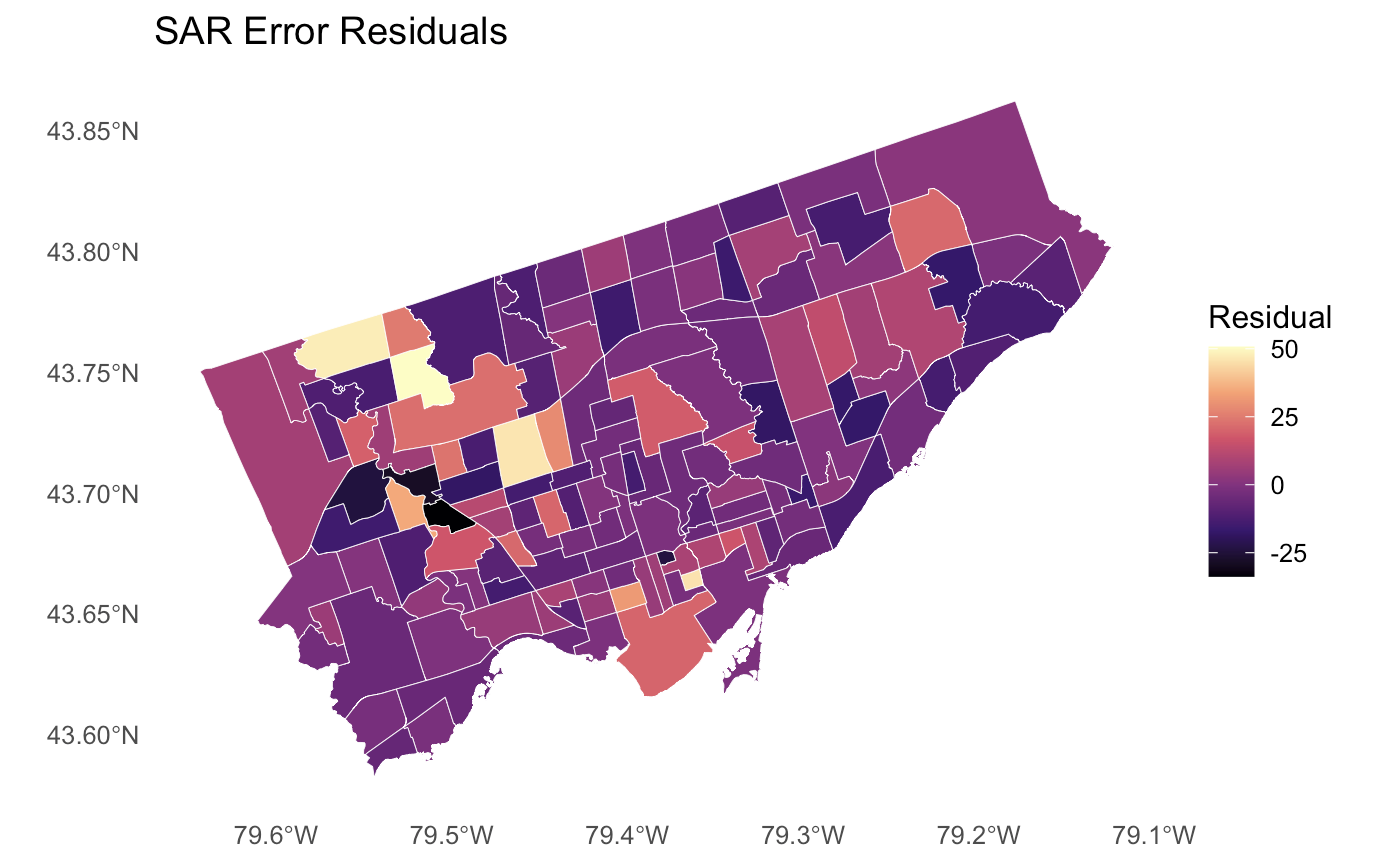
\includegraphics[width=\linewidth]{fig17.png}
\caption{SAR Error}
\end{subfigure}
\hfill
\begin{subfigure}{0.32\textwidth}
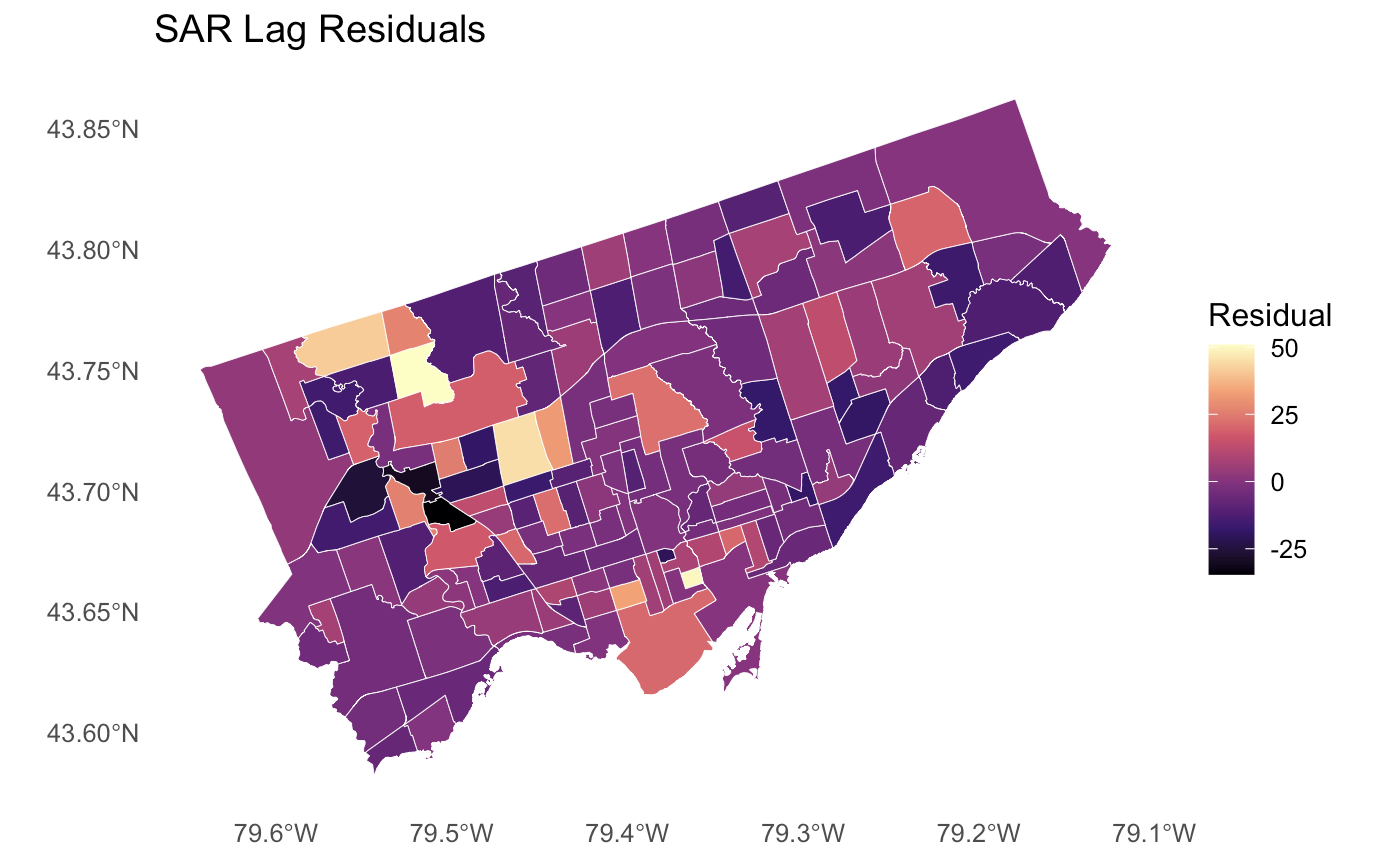
\includegraphics[width=\linewidth]{fig18.png}
\caption{SAR Lag}
\end{subfigure}

\medskip

% ---- Row 2: two models ----
\begin{subfigure}{0.32\textwidth}
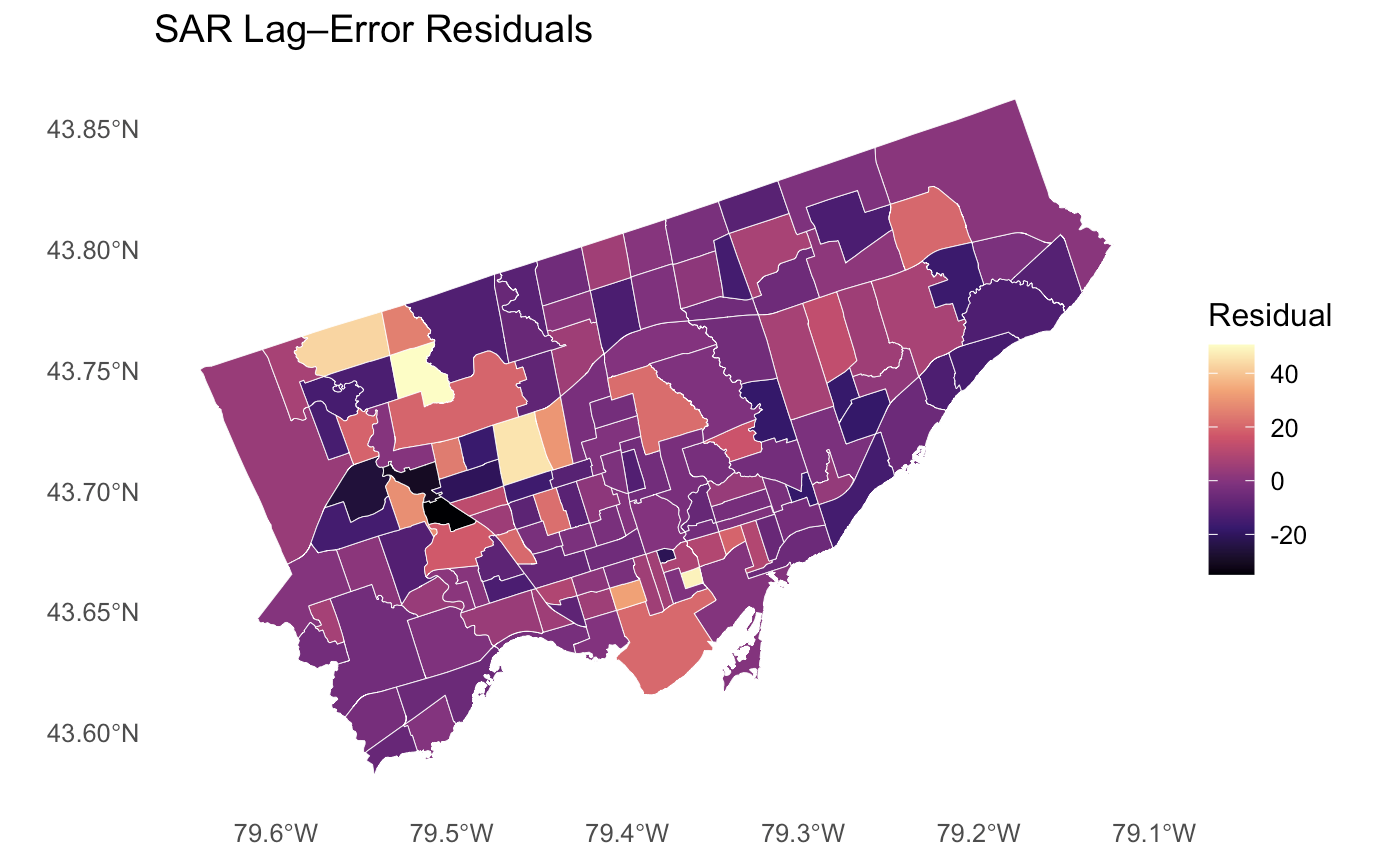
\includegraphics[width=\linewidth]{fig19.png}
\caption{SAR Lag--Error}
\end{subfigure}
\begin{subfigure}{0.32\textwidth}
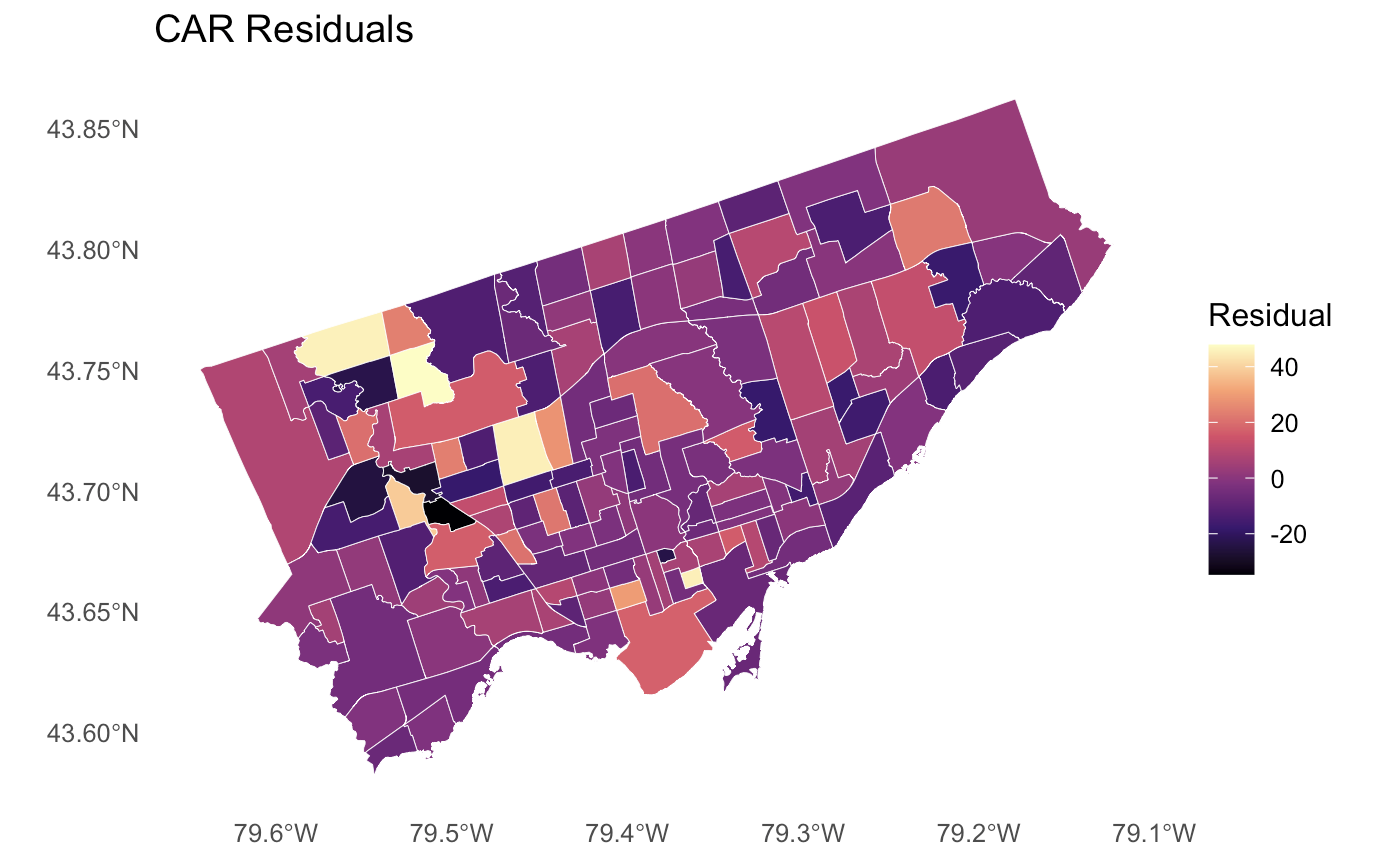
\includegraphics[width=\linewidth]{fig20.png}
\caption{CAR}
\end{subfigure}

\caption{Residual maps for regression models (shooting rate per 10{,}000 residents).}
\label{fig:rq3_residuals}
\end{figure}




\section{Conclusion}

\noindent This project examined the spatial distribution of firearm-related incidents in Toronto using a multi-scale spatial analysis framework. By combining point pattern analysis, neighbourhood-level areal methods, and spatial regression models, we assessed whether firearm violence is randomly distributed across the city, whether neighbourhood-level clustering is present, and whether observed patterns are associated with socioeconomic characteristics.

\noindent Point pattern analysis provided strong evidence against complete spatial randomness, demonstrating that firearm incidents are spatially clustered rather than uniformly distributed across Toronto. These results indicate that incidents are concentrated in specific areas of the city, rather than arising from a purely random spatial process.

\noindent At the neighbourhood level, global and local spatial autocorrelation analyses revealed substantial clustering in shooting rates per 10{,}000 residents. Positive Global Moran’s $I$ values across multiple spatial weight specifications indicate that neighbourhoods with high (or low) shooting rates tend to be located near neighbourhoods with similar rates. Local indicators further showed that elevated rates occur in geographically coherent regions, rather than as isolated neighbourhood-level anomalies. Together, these findings highlight that firearm violence in Toronto exhibits meaningful spatial structure across multiple spatial scales.

\noindent Spatial regression results reinforce these conclusions. Ordinary least squares models exhibited residual spatial autocorrelation, indicating violations of standard regression assumptions. In contrast, spatial models that explicitly accounted for spatial dependence substantially reduced or eliminated residual autocorrelation and improved model fit. Across all models, the proportion of residents identifying as Black was consistently associated with higher neighbourhood-level shooting rates, after controlling for income, unemployment, visible minority composition, and population size. This association should not be interpreted as causal, but rather as reflecting broader structural and historical inequalities that shape spatial patterns of violence.

\noindent Several limitations should be considered when interpreting these findings. First, the analysis relies on police-reported firearm incidents, which may be subject to underreporting or spatial variation in reporting practices \citep{charron2009toronto}. Second, shooting rates were computed using population denominators from the 2021 Census, while incidents span multiple years, implicitly assuming relative population stability over time. Third, neighbourhood-level analyses are subject to the modifiable areal unit problem (MAUP), meaning results may depend on the chosen boundaries. Using aggregated neighbourhood averages also raises the risk of ecological fallacy, as area-level associations may not reflect individual-level relationships. Finally, future work could incorporate temporal dynamics or more flexible models to explore how the relationship between neighbourhood characteristics and firearm violence varies across space.

\noindent Despite these limitations, the consistent evidence of spatial clustering across multiple analytical approaches suggests that the core findings are robust and highlights the importance of spatial analysis for understanding firearm violence in Toronto.

\begin{thebibliography}{99}

\bibitem[Charron(2009)]{charron2009toronto}
Charron, M. (2009).
\textit{Neighbourhood characteristics and the distribution of crime in the City of Toronto}.
Statistics Canada (Catalogue no. 85-561-M, no. 018).
https://www150.statcan.gc.ca/n1/pub/85-561-m/85-561-m2009018-eng.htm


\bibitem[Liu et~al.(2016)]{liu2016changchun}
Liu, D., Song, W., \& Xiu, C. (2016).
Spatial patterns of violent crimes and neighborhood characteristics in Changchun, China.
\textit{Australian \& New Zealand Journal of Criminology, 49}(1), 53--72.
https://doi.org/10.1177/0004865814547133

\bibitem[Zhou et~al.(2023)]{zhou2023london}
Zhou, Y., Wang, F., \& Zhou, S. (2023).
The spatial patterns of the crime rate in London and its socio-economic influence factors.
\textit{Social Sciences, 12}(6), 340.
https://doi.org/10.3390/socsci12060340

\bibitem[Toronto Police Service (n.d.)]{tps_shootings_open_data}
Toronto Police Service. (n.d.).
\textit{Shooting and Firearm Discharges Open Data} [Data set].
Toronto Police Service Public Safety Data Portal.
Retrieved November 10, from https://data.torontopolice.on.ca/datasets/64ddeca12da34403869968ec725e23c4\_0/explore

\bibitem[City of Toronto (n.d.-a)]{city_toronto_neighbourhoods}
City of Toronto. (n.d.-a).
\textit{Neighbourhoods} [Data set].
City of Toronto Open Data Portal.
Retrieved November 10, from https://open.toronto.ca/dataset/neighbourhoods/

\bibitem[City of Toronto (n.d.-b)]{city_toronto_neighbourhood_profiles}
City of Toronto. (n.d.-b).
\textit{Neighbourhood Profiles} [Data set].
City of Toronto Open Data Portal.
Retrieved November 10, 2025, from https://open.toronto.ca/dataset/neighbourhood-profiles/


\end{thebibliography}
\end{document}
